\documentclass[12pt]{article}
\usepackage[margin=2.5cm]{geometry}
\usepackage{enumerate}
\usepackage{amsfonts}
\usepackage{amsmath}
\usepackage{fancyhdr}
\usepackage{amsmath}
\usepackage{amssymb}
\usepackage{amsthm}
\usepackage{mdframed}
\usepackage{graphicx}
\usepackage{subcaption}
\usepackage{adjustbox}
\usepackage{listings}
\usepackage{xcolor}
\usepackage{booktabs}
\usepackage[utf]{kotex}
\usepackage{hyperref}
\usepackage{accents}

\definecolor{codegreen}{rgb}{0,0.6,0}
\definecolor{codegray}{rgb}{0.5,0.5,0.5}
\definecolor{codepurple}{rgb}{0.58,0,0.82}
\definecolor{backcolour}{rgb}{0.95,0.95,0.92}

\lstdefinestyle{mystyle}{
    backgroundcolor=\color{backcolour},
    commentstyle=\color{codegreen},
    keywordstyle=\color{magenta},
    numberstyle=\tiny\color{codegray},
    stringstyle=\color{codepurple},
    basicstyle=\ttfamily\footnotesize,
    breakatwhitespace=false,
    breaklines=true,
    captionpos=b,
    keepspaces=true,
    numbers=left,
    numbersep=5pt,
    showspaces=false,
    showstringspaces=false,
    showtabs=false,
    tabsize=1
}

\lstset{style=mystyle}

\pagestyle{fancy}
\renewcommand{\headrulewidth}{0.4pt}
\lhead{CSC 343}
\rhead{Worksheet 9 Solution}

\begin{document}
\title{CSC343 Worksheet 9 Solution}
\maketitle

\bigskip

\begin{enumerate}[1.]
    \item \textbf{Exercise 11.1.1:}

    \bigskip

    \begin{enumerate}[a)]
        \item

    \begin{center}
    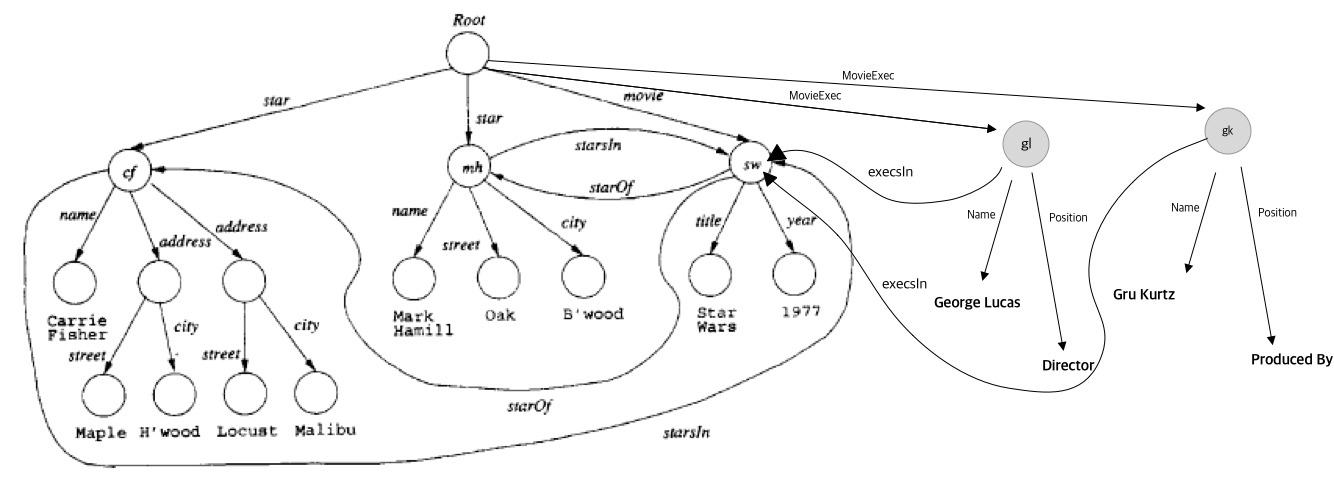
\includegraphics[width=\linewidth]{images/worksheet_9_solution_4.png}
    \end{center}

        \bigskip

        \underline{\textbf{Notes:}}

        \begin{itemize}
            \item Semistructured data
            \begin{itemize}
                \item serves as a model suitable for \textbf{databases integration}, that is,
                for describing the data contained in two or more databases that contain similar data with
                different schemas

                \item It serves as the underlying model for notations such as XML, to be taken
                up in Section 2, that are being used to share information on the web.
            \end{itemize}

            \item Semistructured Data Representation
            \begin{itemize}
                \item is a collection of nodes

            \begin{center}
            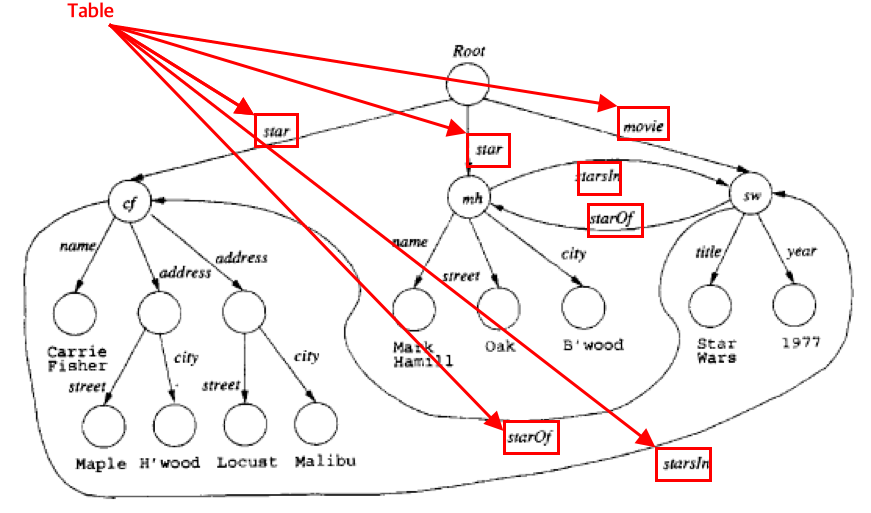
\includegraphics[width=\linewidth]{images/worksheet_9_solution_1.png}
            \end{center}

            \begin{center}
            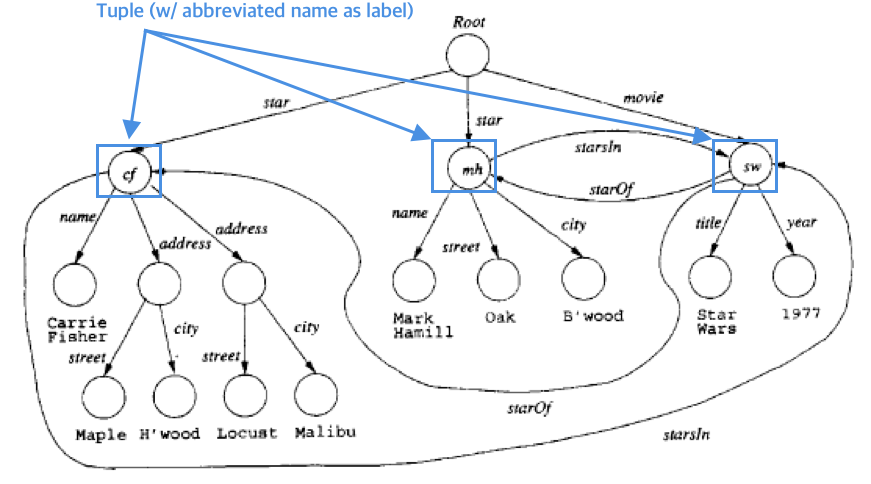
\includegraphics[width=\linewidth]{images/worksheet_9_solution_2.png}
            \end{center}

            \begin{center}
            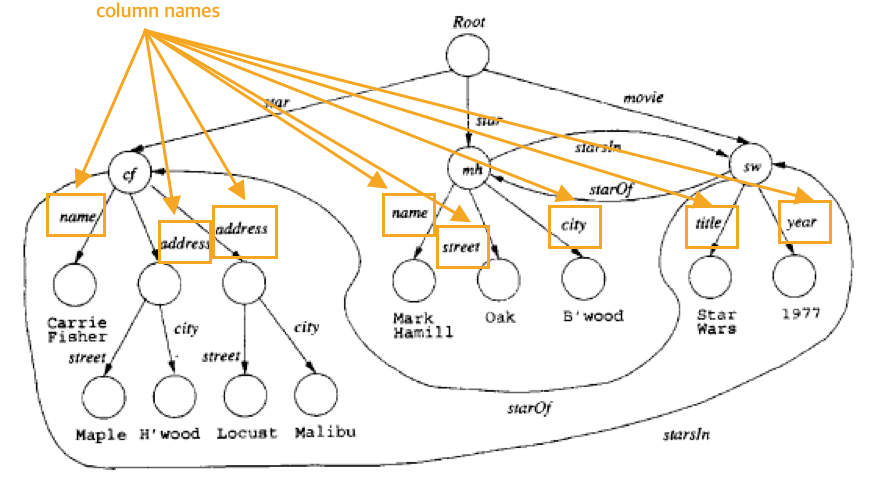
\includegraphics[width=\linewidth]{images/worksheet_9_solution_3.png}
            \end{center}

            \end{itemize}

            \item
        \end{itemize}

        \item

    \begin{center}
    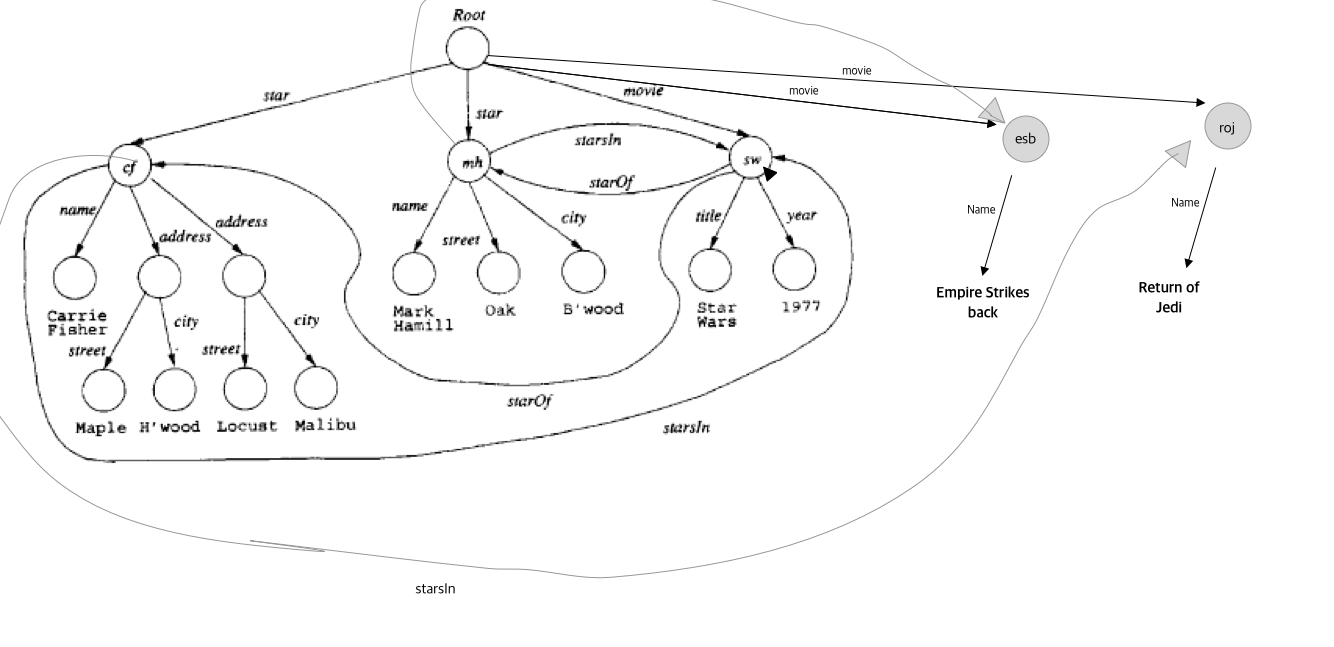
\includegraphics[width=\linewidth]{images/worksheet_9_solution_5.png}
    \end{center}


        \item

    \begin{center}
    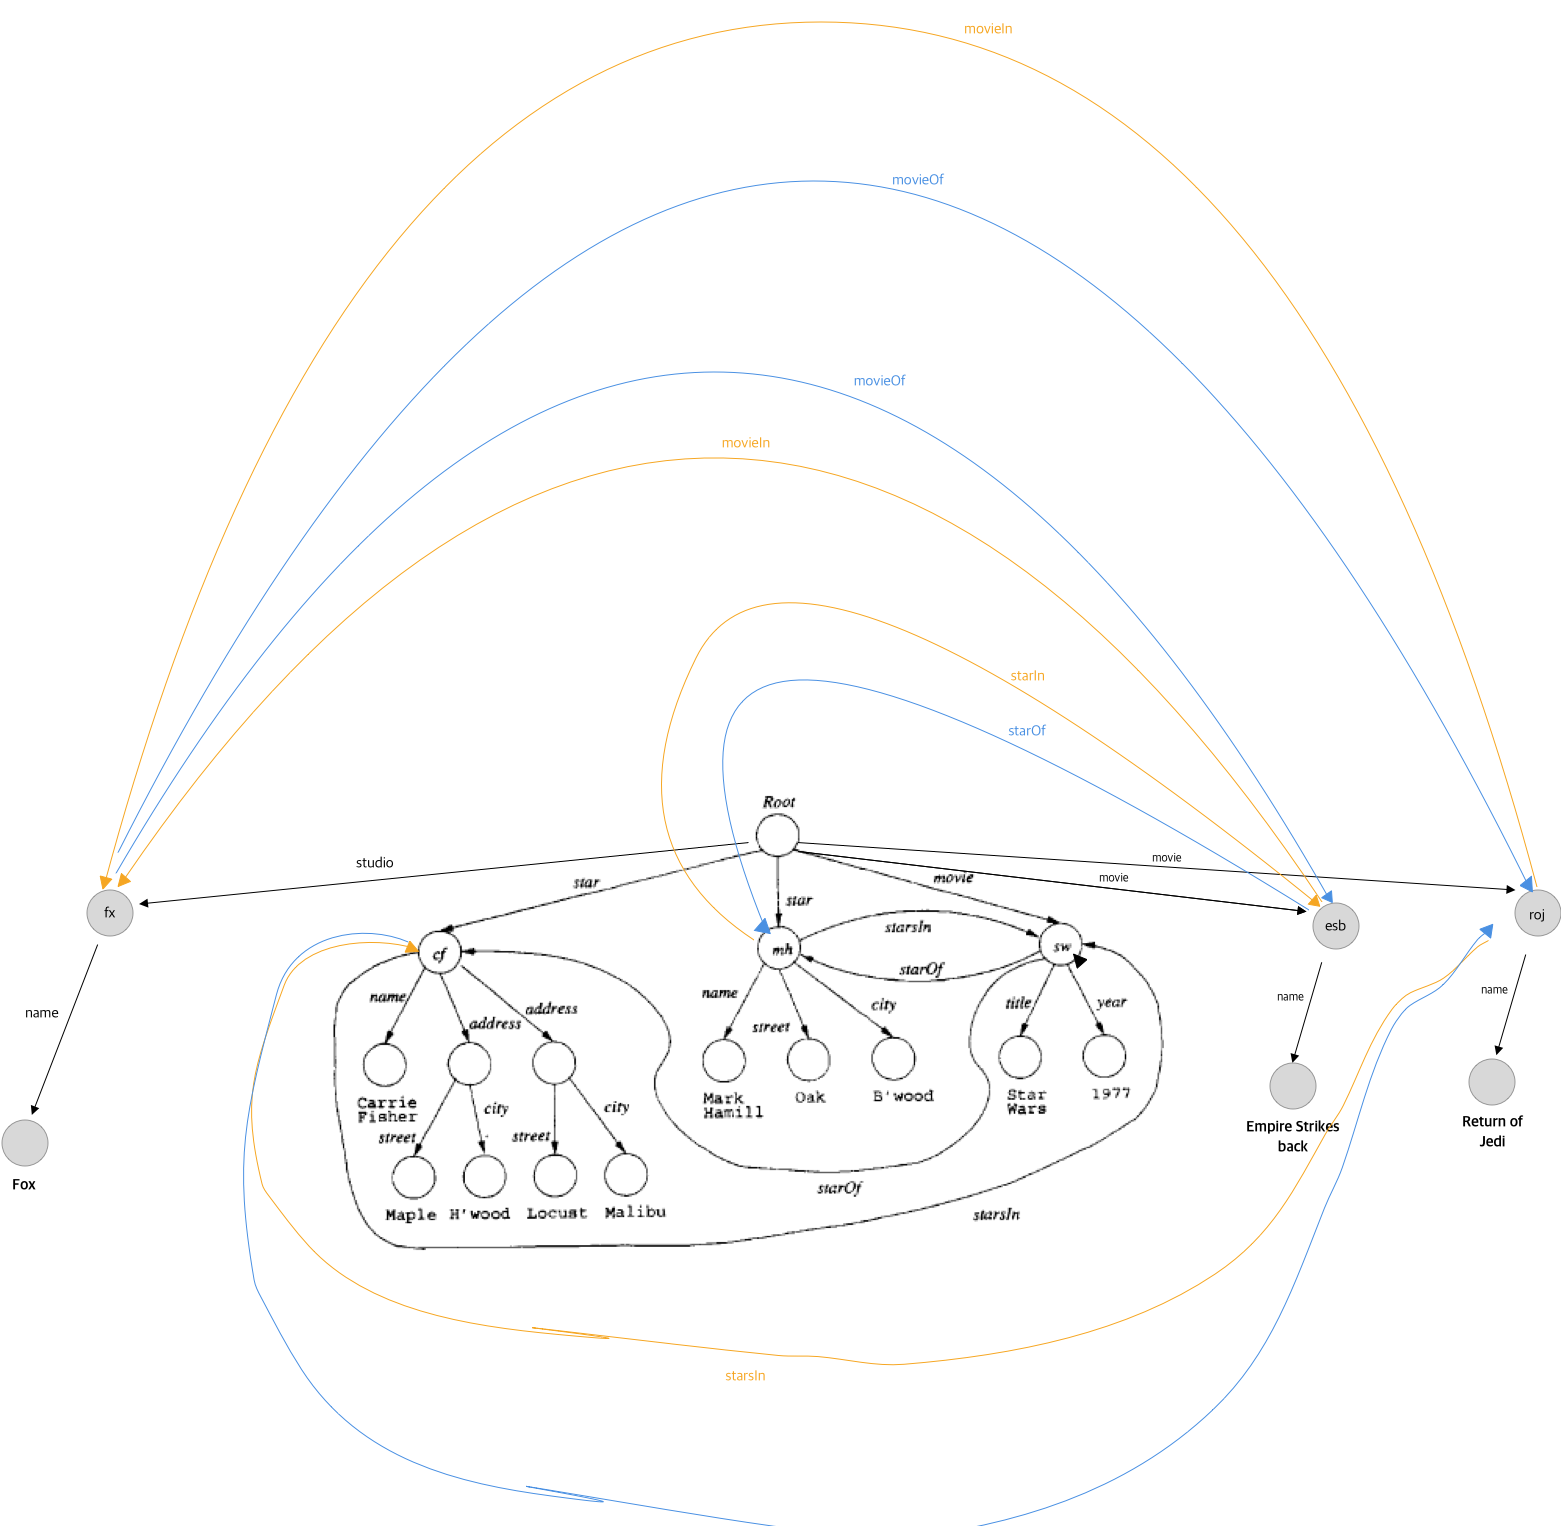
\includegraphics[width=\linewidth]{images/worksheet_9_solution_6.png}
    \end{center}

    \end{enumerate}

    \item

    \begin{center}
    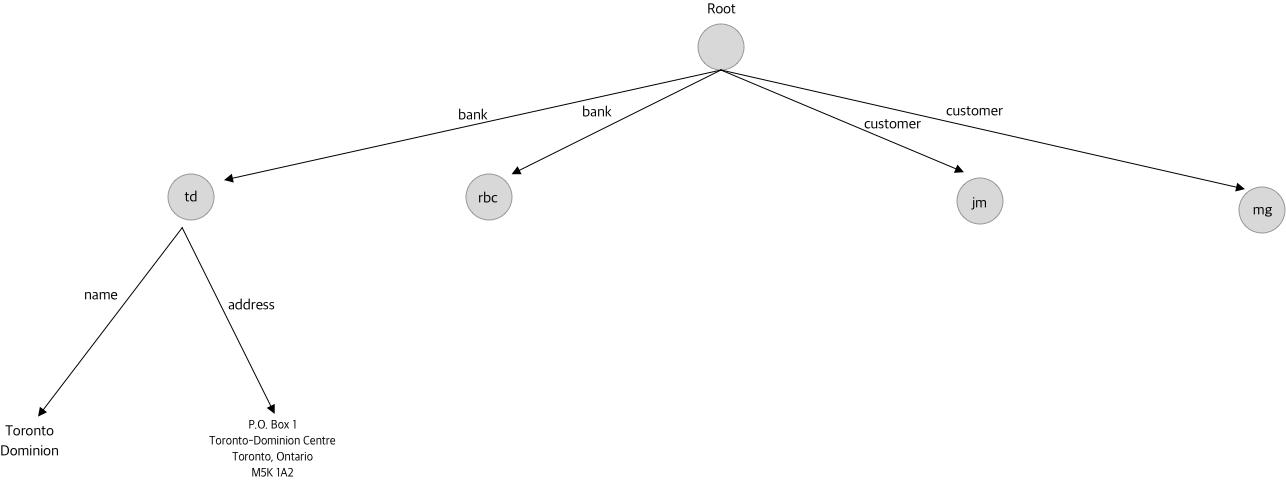
\includegraphics[width=\linewidth]{images/worksheet_9_solution_7.png}
    \end{center}

    \item

    \begin{center}
    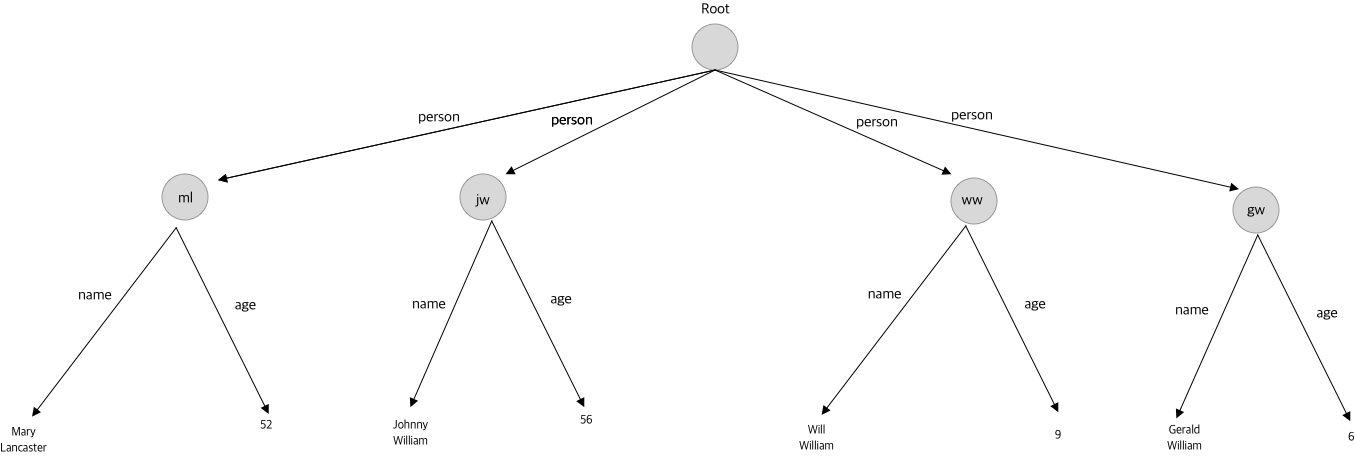
\includegraphics[width=\linewidth]{images/worksheet_9_solution_8.png}
    \end{center}

    \item

    The difference is that UML must fit data into its schema, where as the semi
    structured data allows whatever schema information that is appropriate to be attached to data

    \bigskip

    \underline{\textbf{Notees:}}

    \bigskip

    \begin{itemize}
        \item Semi-structured Data
        \begin{itemize}
            \item Is schemaless
            \item Is motivated primarily by its flexibility
            \item One could enter data at will, and attach to the data whatever schema information
            you felt was appropriate for that data.
            \item Makes query processing harder
        \end{itemize}
        \item Structured Data
        \begin{itemize}
            \item Is rigid framework into which data is placed.
            \item Data must fit into schema
            \item Fixed schema allows data to be organized with data structures
            that support efficient answering of queries
            \item e.g. UML, E/R, Relational, ODL
        \end{itemize}
    \end{itemize}

    \item

    \begin{enumerate}[a)]
        \item

    \begin{lstlisting}[language=XML]
    <? xml version = "1.0" encoding="utf-8" standalone = "yes">
    <StarMovieData>
        <Star starID="cf" starredIn="sw">
            <Name>Carrie Fisher</Name>
            <Address>
                <Street>123 Maple St.</Street>
                <City>Hollywood</City>
            </Address>
            <Address>
                <Street>5 Locust Ln.</Street>
                <City>Malibu</City>
            </Address>
        </Star>
        <Star starID="mh" starredIn="sw">
            <Name>Mark Hamill</Name>
            <Street>456 Oak Rd.</Street>
            <City>Brentwood</City>
        </Star>
        <Movie movieID="sw" starsOf="cf", "mh">
            <Title>Star Wars</Title>
            <Year>1977</Year>
        </Movie>
        <MovieExec movieExecID="gl" execsIn="sw">
            <Name>George Lucas</Name>
            <Position>Director</Position>
        </MovieExec>
        <MovieExec movieExecID="gk" execsIn="sw">
            <Name>Gru Kurtz</Name>
            <Position>Produced By</Position>
        </MovieExec>
    </StarMovieData>
    \end{lstlisting}

        \bigskip

    \begin{itemize}
        \item XML
        \begin{itemize}
            \item is called \textit{Extensible Markup Language}
            \item is an example of semistructured data
        \end{itemize}
        \item XML with and without a Schema
        \begin{itemize}
            \item has two different types
            \begin{enumerate}[1.]
                \item Well-formed XML
                \begin{itemize}
                    \item allows to invent your own tags
                    \item corresponds very-similarly to semi-structured data
                \end{itemize}

                \bigskip

                \underline{\textbf{Example:}}

                \bigskip

    \begin{lstlisting}[language=XML]
    <? xml version = "1.0" encoding="utf-8" standalone = "yes">
    <StarMovieData>
        <Star>
            <Name>Carrie Fisher</Name>
            <Address>
                <Street>123 Maple St.</Street>
                <City>Hollywood</City>
            </Address>
            <Address>
                <Street>5 Locust Ln.</Street>
                <City>Malibu</City>
            </Address>
        </Star>
        <Star>
            <Name>Mark Hamill</Name>
            <Street>456 Oak Rd.</Street>
            <City>Brentwood</City>
        </Star>
        <Movie>
            <Title>Star Wars</Title>
            <Year>1977</Year>
        </Movie>
    </StarMovieData>
    \end{lstlisting}

                \item Valid XML

                \begin{itemize}
                    \item Involes "Document Type Definition"
                    \item specifies allowable tags and gives a grammar for how they may be nested
                \end{itemize}

                \bigskip

            \end{enumerate}
        \end{itemize}

        \item Attributes
        \begin{itemize}
            \item is used to represent connections in a semistructured data graph

            \bigskip

            \underline{\textbf{Example:}}

            \bigskip

    \begin{lstlisting}[language=XML]
    <? xml version = "1.0" encoding="utf-8" standalone = "yes">
    <StarMovieData>
        <Star starID="cf" starredIn="sw">
            <Name>Carrie Fisher</Name>
            <Address>
                <Street>123 Maple St.</Street>
                <City>Hollywood</City>
            </Address>
            <Address>
                <Street>5 Locust Ln.</Street>
                <City>Malibu</City>
            </Address>
        </Star>
        <Star starID="mh" starredIn="sw">
            <Name>Mark Hamill</Name>
            <Street>456 Oak Rd.</Street>
            <City>Brentwood</City>
        </Star>
        <Movie starID="sw" starOf="cf", "mh">
            <Title>Star Wars</Title>
            <Year>1977</Year>
        </Movie>
    </StarMovieData>
    \end{lstlisting}

        \end{itemize}

        \item Namespaces
        \begin{itemize}
            \item \textbf{Syntax:} xmlns:\textit{name}:URI
            \item Is similar to import numpy as np in python
            \item Is used to distinguish tags coming from different sources, i.e. HTML

            \bigskip

            \underline{\textbf{Example:}}

            \bigskip

            Retireving element \textit{StarMovieData} from document \textbf{infolab.stanford.edu/movies}.
            Set md as the name of import

    \begin{lstlisting}[language=XML]
    <md:StarMovieData xmlns:md="http://infolab.stanford.edu/movies">
    \end{lstlisting}
        \end{itemize}
    \end{itemize}

        \item

    \begin{lstlisting}[language=XML]
    <? xml version = "1.0" encoding="utf-8" standalone = "yes">
    <StarMovieData>
        <Star starID="cf" starredIn="sw">
            <Name>Carrie Fisher</Name>
            <Address>
                <Street>123 Maple St.</Street>
                <City>Hollywood</City>
            </Address>
            <Address>
                <Street>5 Locust Ln.</Street>
                <City>Malibu</City>
            </Address>
        </Star>
        <Star starID="mh" starredIn="sw">
            <Name>Mark Hamill</Name>
            <Street>456 Oak Rd.</Street>
            <City>Brentwood</City>
        </Star>
        <Movie movieID="sw" starsOf="cf", "mh">
            <Title>Star Wars</Title>
            <Year>1977</Year>
        </Movie>
        <Movie movieID="esb" starOf="cf", "mh">
            <Title>Empire Strikes Back</Title>
            <Year>1980</Year>
        </Movie>
        <Movie movieID="roj" starOf="cf", "mh">
            <Title>Return of Jedi</Title>
            <Year>1983</Year>
        </Movie>
    </StarMovieData>
    \end{lstlisting}

        \item

    \begin{lstlisting}[language=XML]
    <? xml version = "1.0" encoding="utf-8" standalone = "yes">
    <StarMovieData>
        <Star starID="cf" starredIn="sw">
            <Name>Carrie Fisher</Name>
            <Address>
                <Street>123 Maple St.</Street>
                <City>Hollywood</City>
            </Address>
            <Address>
                <Street>5 Locust Ln.</Street>
                <City>Malibu</City>
            </Address>
        </Star>
        <Star starID="mh" starredIn="sw">
            <Name>Mark Hamill</Name>
            <Street>456 Oak Rd.</Street>
            <City>Brentwood</City>
        </Star>
        <Movie movieID="sw" starsOf="cf", "mh" movieIn="fx">
            <Title>Star Wars</Title>
            <Year>1977</Year>
        </Movie>
        <Movie movieID="esb" starOf="cf", "mh" movieIn="fx">
            <Title>Empire Strikes Back</Title>
            <Year>1980</Year>
        </Movie>
        <Movie movieID="roj" starOf="cf", "mh" movieIn="fx">
            <Title>Return of Jedi</Title>
            <Year>1983</Year>
        </Movie>
        <Studio studioID="fx" movieOf="esb", "roj", "sw">
            <Name>Fox</Name>
            <Address>Hollywood</Address>
        </Studio>
    </StarMovieData>
    \end{lstlisting}

    \end{enumerate}

    \item

    Consider the following relation Classes:

    \begin{center}
    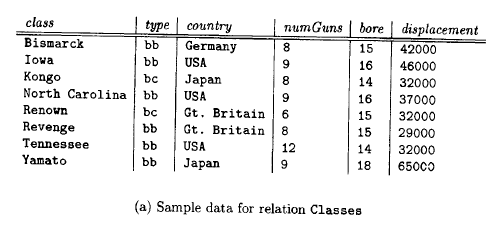
\includegraphics[width=\linewidth]{images/worksheet_9_solution_9.png}
    \end{center}

    \begin{lstlisting}[language=XML]
    <? xml version = "1.0" encoding="utf-8" standalone = "yes">
    <shipsData>
        <Classes>
            <Class>Bismarck</Class>
            <Type>bb</Type>
            <Country>Germany</Country>
            <NumGuns>8</NumGuns>
            <Bore>15</Bore>
            <Displacement>42000</Displacement>
        </Classes>
        <Classes>
            <Class>Iowa</Class>
            <Type>bb</Type>
            <Country>USA</Country>
            <NumGuns>9</NumGuns>
            <Bore>16</Bore>
            <Displacement>46000</Displacement>
        </Classes>
        <Classes>
            <Class>Kongo</Class>
            <Type>bc</Type>
            <Country>Japan</Country>
            <NumGuns>8</NumGuns>
            <Bore>14</Bore>
            <Displacement>32000</Displacement>
        </Classes>
        <Classes>
            <Class>North Carolina</Class>
            <Type>bb</Type>
            <Country>USA</Country>
            <NumGuns>9</NumGuns>
            <Bore>16</Bore>
            <Displacement>37000</Displacement>
        </Classes>
        <Classes>
            <Class>Renown</Class>
            <Type>bc</Type>
            <Country>Gt. Britain</Country>
            <NumGuns>6</NumGuns>
            <Bore>15</Bore>
            <Displacement>32000</Displacement>
        </Classes>
        <Classes>
            <Class>Revenge</Class>
            <Type>bb</Type>
            <Country>Gt. Britain</Country>
            <NumGuns>8</NumGuns>
            <Bore>15</Bore>
            <Displacement>29000</Displacement>
        </Classes>
        <Classes>
            <Class>Tennessee</Class>
            <Type>bb</Type>
            <Country>USA</Country>
            <NumGuns>12</NumGuns>
            <Bore>14</Bore>
            <Displacement>32000</Displacement>
        </Classes>
        <Classes>
            <Class>Yamato</Class>
            <Type>bb</Type>
            <Country>Japan</Country>
            <NumGuns>9</NumGuns>
            <Bore>18</Bore>
            <Displacement>65000</Displacement>
        </Classes>
    </shipsData>
    \end{lstlisting}

        \item

        \bigskip

        \begin{itemize}
            \item DocRoot
    \begin{lstlisting}[language=XML]
    <DocRoot docID="" rootElementID="" />
    \end{lstlisting}
            \item SubElement
    \begin{lstlisting}[language=XML]
    <Subelement parentID="" childID="" position="" />
    \end{lstlisting}
            \item ElementAttribute
    \begin{lstlisting}[language=XML]
    <ElementAttribute elementID="" name="" value="" />
    \end{lstlisting}
            \item ElementValue
    \begin{lstlisting}[language=XML]
    <ElementValue elementID="" name="" value="" />
    \end{lstlisting}
        \end{itemize}

        \bigskip

        \underline{\textbf{Notes:}}

        \bigskip

        \begin{itemize}
            \item Empty element
            \begin{itemize}
                \item is an element that is complete by itself
                \item rather than being composed of a start tag, data
                and an end tag, the empty element is a combined start and end tag.

                \bigskip

                \underline{\textbf{Example:}}

                \bigskip

    \begin{lstlisting}[language=XML]
    <phone>
        <entry>
            <name>Chip</name>
            <extension number="3"/>
        </entry>
    </phone>
    \end{lstlisting}

                \bigskip

                \begin{itemize}
                    \item Phone is not an empty element
                    \item extension is an empty element
                \end{itemize}
            \end{itemize}
    \end{itemize}

    \item

    \bigskip

    The following will be used as an example.

    \bigskip

    \begin{center}
    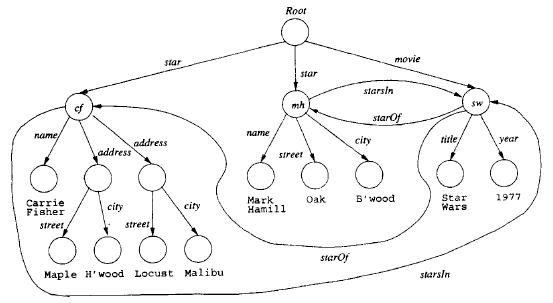
\includegraphics[width=\linewidth]{images/worksheet_9_solution_10.png}
    \end{center}

    \bigskip

    \begin{lstlisting}[language=XML]
    <? xml version = "1.0" encoding="utf-8" standalone = "yes">
    <DocRoot docID="root" rootElementID="">
        <SubElement parentID="root" childID="cf" position="1">
            <ElementAttribute elementID="cf-starsIn" name="starsIn" value="sw"/>
            <ElementValue elementID="cf-name" name="name" value="Carrie Fisher"/>
            <SubElement parentID="cf" childID="cf-add_1" position="1">
                <City elementID="cf-add_1-city" value="Hollywood">
                <Street elementID="cf-add_1-street" value="Maple">
            </SubElement>
            <SubElement parentID="cf" childID="cf-add_2" position="2">
                <ElementValue elementID="cf-add_2-city" value="Malibu">
                <ElementValue elementID="cf-add_1-street" value="Locust">
            </SubElement>
        </SubElement>
        <SubElement parentID="root" childID="mh" position="2">
            <ElementAttribute elementID="mh-starsIn" name="starsIn" value="sw"/>
            <ElementValue elementID="mh-name" value="Mark Hamill"/>
            <SubElement parentID="mh" childID="mh-add_2" position="1">
                <ElementValue elementID="mh-add_2-city" value="Bollywood">
                <ElementValue elementID="mh-add_2-street" value="Oak">
            </SubElement>
        </SubElement>
        <SubElement parentID="root" childID="sw" position="3">
            <ElementAttribute elementID="mh-starsOf_1" name="starsOf" value="cf"/>
            <ElementAttribute elementID="mh-starsOf_2" name="starsOf" value="mh"/>
            <ElementValue elementID="sw-title" value="Star Wars" />
            <ElementValue elementID="sw-year" value="1977" />
        </SubElement>
    </DocRoot>
    \end{lstlisting}

    \item

    \begin{enumerate}[a)]
        \item
    \begin{lstlisting}[language=XML]
    <? xml version = "1.0" encoding="utf-8" standalone = "yes">
    <StarMovieData>
        <Star starID="cf" starredIn="sw">
            <Name>Carrie Fisher</Name>
            <Address>
                <Street>123 Maple St.<Street>
                <City>Hollywood</City>
            </Address>
            <Address>
                <Street>5 Locust Ln.</Street>
                <City>Malibu</City>
            </Address>
        </Star>
        <Star starID="mh" starredIn="sw">
            <Name>Mark Hamill</Name>
            <Address>
                <Street>456 Oak Rd.</Street>
                <City>Brentwood</City>
            </Address>
        </Star>
        <Movie movieID="sw" starsOf="cf mh">
            <Title>Star Wars</Title>
            <Year>1977</Year>
        </Movie>
        <Movie movieID="esb" starsOf="cf mh">
            <Title>The Empire Strikes Back</Title>
            <Year>1980</Year>
        </Movie>
        <Movie movieID="roj" starsOf="cf mh">
            <Title>Return of the Jedi</Title>
            <Year>1983</Year>
        </Movie>
    </StarMovieData>
    \end{lstlisting}
        \item

    \begin{lstlisting}[language=XML]
    <? xml version = "1.0" encoding="utf-8" standalone = "yes">
    <StarMovieData>
        <Star starID="cf" starredIn="sw">
            <Name>Carrie Fisher</Name>
            <Address>
                <Street>123 Maple St.<Street>
                <City>Hollywood</City>
            </Address>
            <Address>
                <Street>5 Locust Ln.</Street>
                <City>Malibu</City>
            </Address>
        </Star>
        <Star starID="hf" starredIn="sw fw">
            <Name>Harrison Ford</Name>
        </Star>

        <Star starID="mh" starredIn="sw">
            <Name>Mark Hamill</Name>
            <Address>
                <Street>456 Oak Rd.</Street>
                <City>Brentwood</City>
            </Address>
        </Star>
        <Movie movieID="sw" starsOf="cf mh hf">
            <Title>Star Wars</Title>
            <Year>1977</Year>
        </Movie>
        <Movie movieID="esb" starsOf="cf mh hf">
            <Title>The Empire Strikes Back</Title>
            <Year>1980</Year>
        </Movie>
        <Movie movieID="roj" starsOf="cf mh hf">
            <Title>Return of the Jedi</Title>
            <Year>1983</Year>
        </Movie>
        <Movie movieID="fw" starsOf="hf">
            <Title>Firewall</Title>
            <Year>2006</Year>
        </Movie>
    </StarMovieData>
    \end{lstlisting}

        \item

    \begin{lstlisting}[language=XML]
    <? xml version = "1.0" encoding="utf-8" standalone = "yes">
    <StarMovieData>
        <Star starID="cf" starredIn="sw">
            <Name>Carrie Fisher</Name>
            <Address>
                <Street>123 Maple St.<Street>
                <City>Hollywood</City>
            </Address>
            <Address>
                <Street>5 Locust Ln.</Street>
                <City>Malibu</City>
            </Address>
        </Star>
        <Star starID="hf" starredIn="sw fw">
            <Name>Harrison Ford</Name>
        </Star>

        <Star starID="mh" starredIn="sw">
            <Name>Mark Hamill</Name>
            <Address>
                <Street>456 Oak Rd.</Street>
                <City>Brentwood</City>
            </Address>
        </Star>
        <Movie movieID="sw" starsOf="cf mh hf">
            <Title>Star Wars</Title>
            <Year>1977</Year>
        </Movie>
        <Movie movieID="esb" starsOf="cf mh hf">
            <Title>The Empire Strikes Back</Title>
            <Year>1980</Year>
        </Movie>
        <Movie movieID="roj" starsOf="cf mh hf">
            <Title>Return of the Jedi</Title>
            <Year>1983</Year>
        </Movie>
        <Movie movieID="fw" starsOf="hf">
            <Title>Firewall</Title>
            <Year>2006</Year>
        </Movie>
        <Movie movieID="hhs" starsOf="cf">
            <Title>Hannah and Her Sisters</Title>
            <Year>1985</Year>
        </Movie>
    </StarMovieData>
    \end{lstlisting}

        \item

    \begin{lstlisting}[language=XML]
    <? xml version = "1.0" encoding="utf-8" standalone = "yes">
    <StarMovieData>
        <Star starID="cf" starredIn="sw">
            <Name>Carrie Fisher</Name>
            <Address>
                <Street>123 Maple St.<Street>
                <City>Hollywood</City>
            </Address>
            <Address>
                <Street>5 Locust Ln.</Street>
                <City>Malibu</City>
            </Address>
        </Star>
        <Star starID="hf" starredIn="sw fw">
            <Name>Harrison Ford</Name>
        </Star>
        <Star starID="mh" starredIn="sw">
            <Name>Mark Hamill</Name>
            <Address>
                <Street>456 Oak Rd.</Street>
                <City>Brentwood</City>
            </Address>
        </Star>
        <Star starID="md" starredIn="bi">
            <Name>Matt Damon</Name>
        </Star>
        <Movie movieID="sw" starsOf="cf mh hf">
            <Title>Star Wars</Title>
            <Year>1977</Year>
        </Movie>
        <Movie movieID="esb" starsOf="cf mh hf">
            <Title>The Empire Strikes Back</Title>
            <Year>1980</Year>
        </Movie>
        <Movie movieID="roj" starsOf="cf mh hf">
            <Title>Return of the Jedi</Title>
            <Year>1983</Year>
        </Movie>
        <Movie movieID="fw" starsOf="hf">
            <Title>Firewall</Title>
            <Year>2006</Year>
        </Movie>
        <Movie movieID="hhs" starsOf="cf">
            <Title>Hannah and Her Sisters</Title>
            <Year>1985</Year>
        </Movie>
        <Movie movieID="bi" starsOf="md">
            <Title>The Bourne Identity</Title>
            <Year>2002</Year>
        </Movie>
    </StarMovieData>
    \end{lstlisting}

    \end{enumerate}

    \item

    \begin{lstlisting}[language=XML]
    <!DOCTYPE BankData [
        <!ELEMENT BankData (Accounts*, Customers*)>
        <!ELEMENT Accounts(acctNo, type, balance)>
            <!ATTLIST Accounts
                acctNo ID #REQUIRED
                acctIn IDREFS #IMPLIED
            >
        <!ELEMENT Customers(firsrName, lastName, idNo, account)>
            <!ATTLIST Accounts
                idNo ID #REQUIRED
                account IDREFS #IMPLIED
            >
        <!ELEMENT acctNo (#PCDATA)>
        <!ELEMENT type (#PCDATA)>
        <!ELEMENT balance (#PCDATA)>
        <!ELEMENT firstName (#PCDATA)>
        <!ELEMENT lastName (#PCDATA)>
        <!ELEMENT idNo (#PCDATA)>
        <!ELEMENT account (#PCDATA)>
    ]>
    \end{lstlisting}

    \bigskip

    \begin{mdframed}

    \underline{\textbf{Correct Solution:}}

    \bigskip

    \begin{lstlisting}[language=XML]
    <!DOCTYPE BankData [
        <!ELEMENT BankData (Accounts*, Customers*)>
        <!ELEMENT Accounts(acctNo, type, balance)>
            <!ATTLIST Accounts
                acctNo ID #REQUIRED
                acctIn IDREFS #IMPLIED
            >
        <!ELEMENT Customers(firsrName, lastName, idNo, account)>
            <!ATTLIST Accounts
                idNo ID #REQUIRED
                account IDREFS #IMPLIED
            >
        <!ELEMENT acctNo (#PCDATA)>
        <!ELEMENT type (#PCDATA)>
        <!ELEMENT balance (#PCDATA)>
        <!ELEMENT firstName (#PCDATA)>
        <!ELEMENT lastName (#PCDATA)>
        <!ELEMENT idNo (#PCDATA)>
        <!ELEMENT account (#PCDATA)>
    ]>
    \end{lstlisting}

    \end{mdframed}

    \item

    \begin{lstlisting}[language=XML]
    <!DOCTYPE TeamData [
        <!ELEMENT TeamData (Players*, Teams*, Fans*)>
        <!ELEMENT Players(FirstName, LastName, Team)>
            <!ATTLIST Players
                playerId ID #REQUIRED
                playerIn IDREFS #IMPLIED
            >
        <!ELEMENT FirstName (#PCDATA)>
        <!ELEMENT LastName (#PCDATA)>
        <!ELEMENT Team (#PCDATA)>
        <!ELEMENT Teams(Name)>
            <!ATTLIST Teams
                teamId ID #REQUIRED
                playerOf IDREFS #IMPLIED
                fanOf IDREFS #IMPLIED
            >
        <!ELEMENT Name (#PCDATA)>
        <!ELEMENT Fans(FirstName, LastName)>
            <!ATTLIST Fans
                faId ID #REQUIRED
                fanIn IDREFS #IMPLIED
            >
    ]>
    \end{lstlisting}

    \bigskip

    \underline{\textbf{Notes:}}

    \begin{itemize}
        \item There is no need to write same tags twice. (e.g. FirstName, LastName)
    \end{itemize}

    \item

    \begin{lstlisting}[language=XML]
    <!DOCTYPE GenealogyData [
        <!ELEMENT GenealogyData (Person)>
        <!ELEMENT Person(FirstName, LastName, Age)>
            <!ATTLIST Person
                personId ID #REQUIRED
                spouse IDREFS #IMPLIED
                husband IDREFS #IMPLIED
                child IDREFS #IMPLIED
                brother IDREFS #IMPLIED
            >
        <!ELEMENT FirstName (#PCDATA)>
        <!ELEMENT LastName (#PCDATA)>
    ]>
    \end{lstlisting}


    \bigskip

    \underline{\textbf{Notes:}}

    \bigskip

    \begin{itemize}
        \item PCDATA
        \begin{itemize}
            \item Is text that will be parsed by a parser.
            \item Tags inside the text will be treated as markup and entities will be expanded.
        \end{itemize}
        \item CDATA
        \begin{itemize}
            \item Is text that will not be parsed by a parser.
            \item Tags inside the text will not be treated as markup and entities will not be expanded
            \item e.g. attributes

    \begin{lstlisting}[language=XML]
    <Movie title="Star Wars" year="1977" genre="sciFi">

    <!ELEMENT Movie EMPTY>
        <!ATTLIST Movie
            title CDATA #REQUIRED
            year  CDATA #REQUIRED
            genre (comedy | drama | sciFi | teen) #IMPLIED
        >

    \end{lstlisting}
        \end{itemize}
    \end{itemize}

    \item

    \begin{lstlisting}[language=XML]
    <!DOCTYPE ShipBattleData [

    ]>
    \end{lstlisting}

    \item

    \begin{itemize}
        \item An example of a document that conforms tothe XML Schema


    \begin{lstlisting}[language=XML]
    <? xml version = "1.0" encoding = "utf-8" ?>
    <Movies>
        <Movie>
            <Title>Star Wars</Title>
            <Year>1977</Year>
        </Movie>
        <Movie>
            <Title>Return of the Jedi</Title>
            <Year>1983</Year>
        </Movie>
    </Movies>
    \end{lstlisting}

        \item An example of one that has all the elements mentioned, but does not conform to
        definition

    \begin{lstlisting}[language=XML]
    <? xml version = "1.0" encoding = "utf-8" ?>
    <Movies>
        <Movie>
            <Title>Star Wars</Title>
            <Year>1977</Year>
        </Movie>
        <Movie>
            <Title>Return of the Jedi</Title>
            <Year>This is not correct</Year>
        </Movie>
    </Movies>
    \end{lstlisting}


    \end{itemize}

    \bigskip

    \underline{\textbf{Notes:}}

    \bigskip

    \begin{itemize}
        \item XML Schema
        \begin{itemize}
            \item is an alternative way to provide a schema for XML documents
            \item is more powerful than DTD
            \begin{itemize}
                \item allows to declare types such as integer or float
                \item gives ability to declare keys and foreign keys
            \end{itemize}
        \end{itemize}

        \item The Form of an XML Schema
        \begin{itemize}
            \item Each XML-Schema document has the form

            \bigskip

            $<$? xml version = "1.0" encoding = "utf-8" ?$>$

            $<$xs:schema xmlns:xs="http://www.w3.org/2001/XMLSchema"$>$

            \quad...

            $<$/xs:schema$>$

        \end{itemize}
        \item Elements
        \begin{itemize}
            \item \textbf{Syntax:}

            \bigskip

            $<$xs:element name = element name type = element type$>$

            \quad\textit{constraints and / or structure information}

            $<$/xs:element$>$


        \bigskip

        \underline{\textbf{Example:}}

        \bigskip

    \begin{lstlisting}[language=XML]
    <xs:element name = "title" type = "xs:string" />
    <xs:element name = "Year" type = "xs:integerg" />

    \end{lstlisting}

        \end{itemize}

        \item Complex Types
        \begin{itemize}
            \item is an XML element that contains other elements and/or attributes. $^{[1]}$
            \item \textbf{Syntax:}

            \bigskip

            $<$xs:complexType name = \textit{type name}$>$

            \quad$<$xs:sequence$>$

            \quad\quad\textit{list of element definitions}

            \quad$<$/xs:sequence$>$

            $<$/xs:complexType$>$
        \end{itemize}

        \bigskip

        \underline{\textbf{Example:}}

        \bigskip

    \begin{lstlisting}[language=XML]
    <? xml version = "1.0" encoding = "utf-8" ?>
    <xs:schema xmlns:xs = "http://www.w3.org/2001/XMLSchema">

        <xs:complexType name = "movieType">
            <xs:sequence>
                <xs:element name = "Title" type = "xs:string" />
                <xs:element name = "year" type = "xs:integer" />
            </xs:sequence>
        </xs:complexType>

        <xs:element name = "Movies">
            <xs:complexType>
                <xs:sequence>
                    <xs:element name="Movie" type="movieType" minOccurs="0" maxOccurs = "unbounded" />
                </xs:sequence>
            </xs:complexType>
        </xs:element>
    </xs:schema>
    \end{lstlisting}

        \item Complex Types Attributes
        \begin{itemize}
            \item \textbf{Syntax:}

            $<$xs:attribute name = \textit{attribute name} type = \textit{type name} \textit{other information about the attribute} /$>$


            \bigskip

            \begin{itemize}
                \item \textit{other information} includes

                \begin{enumerate}[1.]
                    \item default value
                    \item required
                    \item type
                \end{enumerate}
            \end{itemize}


            \bigskip

            \underline{\textbf{Example:}}

            \bigskip

            \begin{center}
            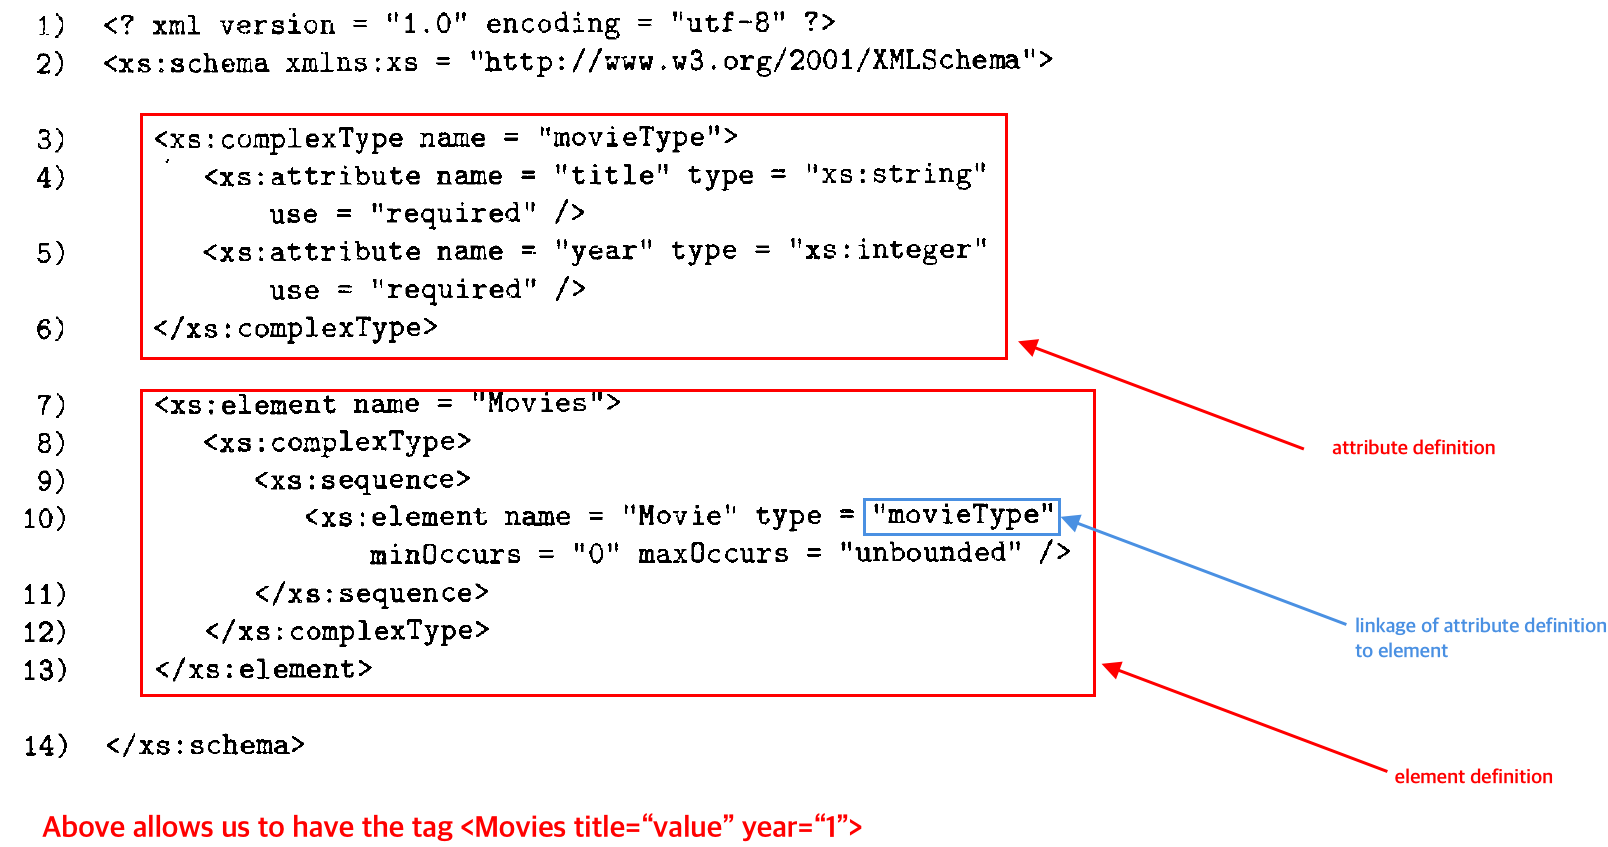
\includegraphics[width=\linewidth]{images/worksheet_9_solution_11.png}
            \end{center}

        \end{itemize}

        \item Restricted Simple Types
        \begin{itemize}
            \item Can be used as an attribute or element
            \begin{enumerate}[1.]
                \item Restricting numerical values by \underline{setting lower bound and upperbound}
                \begin{itemize}
                    \item \textbf{Syntax:}

                    \bigskip

                    $<$xs:simpleType name = \textit{type name}$>$

                    \quad$<$xs:restriction base = \text{base type} $>$

                    \quad\quad\textit{upper and/or lower bounds}

                    \quad$<$/xs:restriction $>$

                    $<$/xs:simpleType$>$

                    \item Use \textbf{minInclusive} to state the lower bound
                    \item Use \textbf{maxInclusive} to state the upper bound
                \end{itemize}

                \bigskip

                \underline{\textbf{Example:}}

                \bigskip

    \begin{lstlisting}[language=XML]
    <xs:simpleType name = "movieYearType">
        <xs:restriction base = "xs:integer">
            <xs:minInclusive value = "1915" />
        </xs:restriction>
    </xs:simpleType>
    \end{lstlisting}
                \item Restricting values to an \underline{enumerated} type
                \begin{itemize}
                    \item \textbf{Syntax:}

                    \bigskip

                    $<$xs:simpleType name = "movieYearType" $>$

                    \quad$<$xs:restriction base = "xs:string"$>$

                    \quad\quad$<$xs:enumeration value = "comedy"$/>$

                    \quad\quad$<$xs:enumeration value = "drama"$/>$

                    \quad\quad$<$xs:enumeration value = "sciFi"$/>$

                    \quad\quad$<$xs:enumeration value = "teen"$/>$

                    \quad$<$/xs:restriction$>$

                    $<$/xs:simpleType$>$
                \end{itemize}

                \bigskip

                \underline{\textbf{Example:}}

                \bigskip

    \begin{lstlisting}[language=XML]
    <xs:simpleType name = "genreType">
        <xs:restriction base = "xs:string">
            <xs:enumeration value = "comedy"/>
            <xs:enumeration value = "drama"/>
            <xs:enumeration value = "sciFi"/>
            <xs:enumeration value = "teen"/>
        </xs:restriction>
    </xs:simpleType>
    \end{lstlisting}
            \end{enumerate}
        \end{itemize}

        \item Keys in XML Schema
        \begin{itemize}
            \item \textbf{Syntax:}

            $<$xs:key name = \textit{key name}$>$

            \quad$<$xs:selector xpath= \textit{path description} $>$

            \quad$<$xs:field xpath = \textit{path description} $>$

            $<$/xs:key$>$

            \bigskip

            \underline{\textbf{Example:}}

            \bigskip

            \begin{center}
            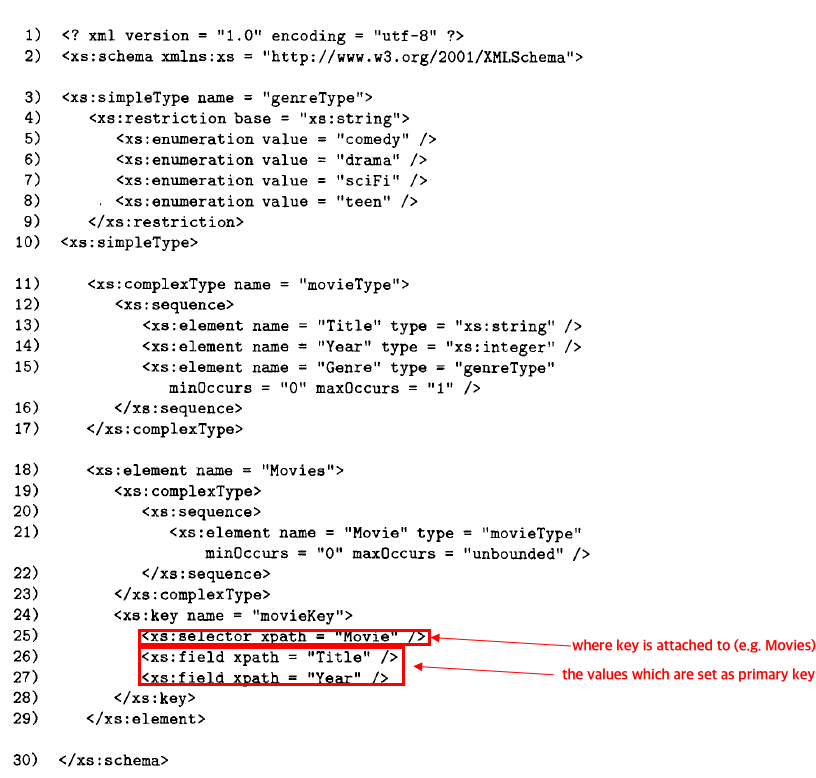
\includegraphics[width=\linewidth]{images/worksheet_9_solution_12.png}
            \end{center}

            \item XPath of element $\to$ \textit{element name}

    \begin{center}
    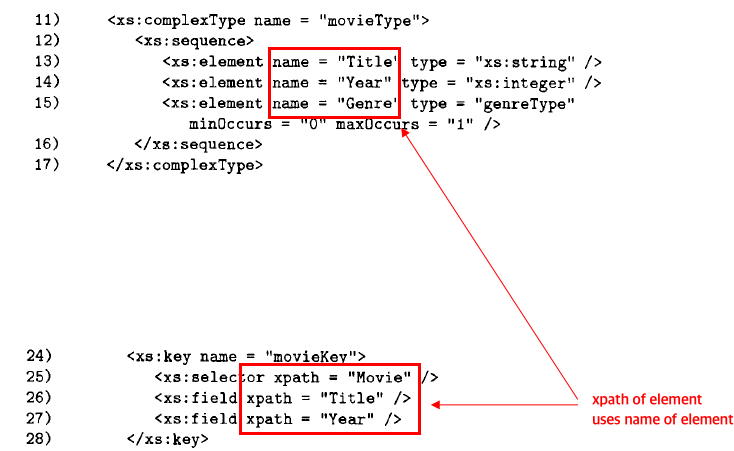
\includegraphics[width=\linewidth]{images/worksheet_9_solution_14.png}
    \end{center}

            \item XPath of attribute $\to$ @\textit{attribute name}

            \bigskip


    \begin{center}
    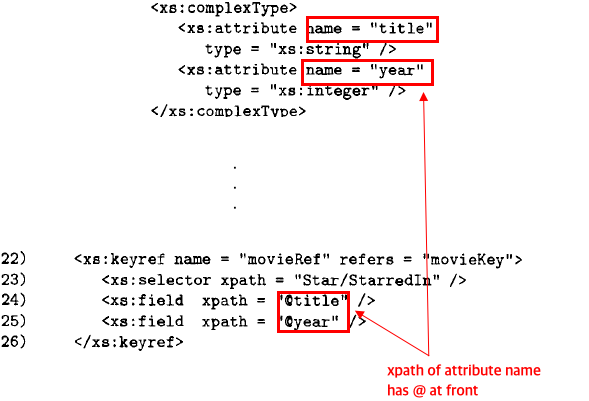
\includegraphics[width=\linewidth]{images/worksheet_9_solution_13.png}
    \end{center}

        \end{itemize}

        \item Foreign Keys in XML Schema
        \begin{itemize}
            \item \textbf{Syntax:}

            \bigskip

            $<$xs:keyref name = \textit{foreign-key name} refer = \textit{key name} $>$

            \quad$<$xs:selector xpath = \textit{path description} $>$

            \quad$<$xs:field xpath = \textit{path description} $>$

            $<$/xs:keyref $>$
        \end{itemize}
    \end{itemize}

    \bigskip

    \underline{\textbf{References:}}

    \bigskip

    \begin{enumerate}[1.]
        \item w3School : Complex Type, \href{https://www.w3schools.com/xml/el_complextype.asp}{link}
    \end{enumerate}

    \item

    \begin{lstlisting}[language=XML]
    <? xml version = "1.0" encoding = "utf-8" ?>
    <xs:schema xmlns:xs = "http://www.w3.org/2001/XMLSchema">

        <xs:complexType name = "movieType">
            <xs:sequence>
                <xs:element name = "Title" type = "xs:string" />
                <xs:element name = "year" type = "xs:integer" />
            </xs:sequence>
        </xs:complexType>

        <xs:element name = "Movies">
            <xs:complexType>
                <xs:sequence>
                    <xs:element name="NotMovie" type="movieType" minOccurs="0" maxOccurs = "unbounded" /> // <- Corrected
                </xs:sequence>
            </xs:complexType>
        </xs:element>
    </xs:schema>
    \end{lstlisting}

\end{enumerate}

\end{document}